\documentclass{article}
\usepackage{pgfplots}
\pgfplotsset{compat=1.18}

\begin{document}

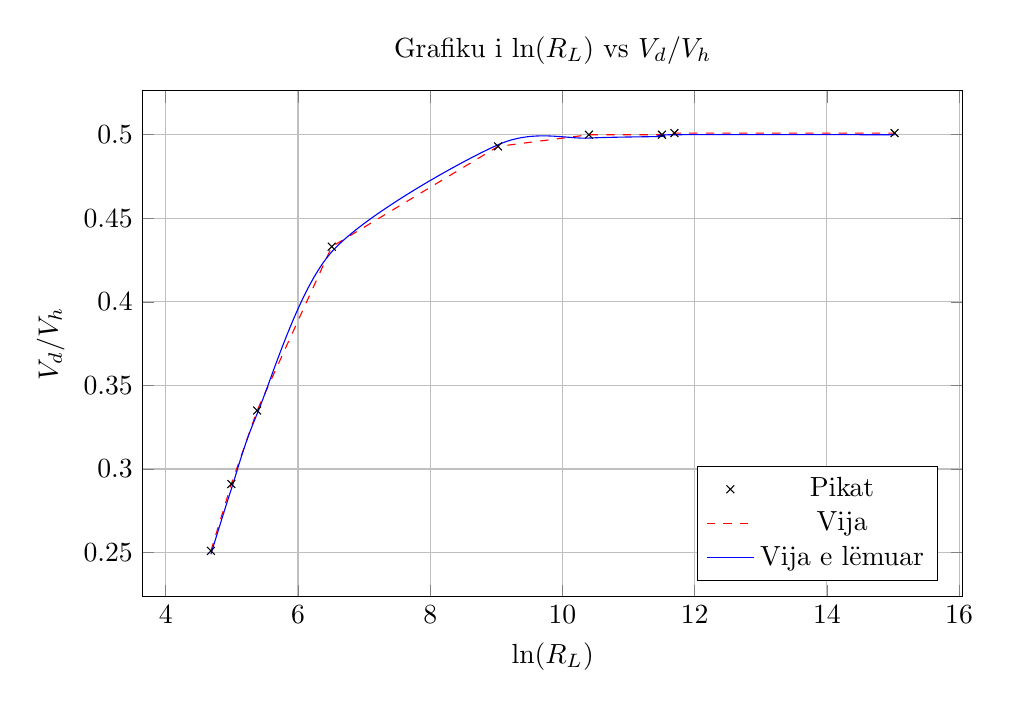
\begin{tikzpicture}
    \begin{axis}[
        xlabel={$\ln(R_L)$},
        ylabel={$V_d/V_h$},
        title={Grafiku i $\ln(R_L)$ vs $V_d/V_h$},
        grid=major,
        legend pos=south east,
        width=12cm,
        height=8cm
    ]
    %Pikat
    \addplot[only marks, black, mark=x] coordinates {
        (4.683, 0.251)
        (4.992, 0.291)
        (5.382, 0.335)
        (6.511, 0.433)
        (9.026, 0.493)
        (10.401, 0.5)
        (11.506, 0.5)
        (11.695, 0.501)
        (15.024, 0.501)
    };
    \addlegendentry{Pikat}

    %Vija e kuqe
    \addplot[red, dashed] coordinates {
        (4.683, 0.251)
        (4.992, 0.291)
        (5.382, 0.335)
        (6.511, 0.433)
        (9.026, 0.493)
        (10.401, 0.5)
        (11.506, 0.5)
        (11.695, 0.501)
        (15.024, 0.501)
    };
    \addlegendentry{Vija}

    % Vija e lemuar
    \addplot[blue, thin, smooth] coordinates {
        (4.683, 0.249)
        (4.992, 0.288)
        (5.382, 0.333)
        (6.512, 0.430)
        (9.026, 0.494)
        (10.401, 0.498)
        (11.507, 0.499)
        (11.695, 0.5)
        (15.024, 0.5)
    };
    \addlegendentry{Vija e lëmuar}

    \end{axis}
\end{tikzpicture}
\end{document}